
\title{Programmierung}
\subtitle{Einführungsübung}

\begin{document}
    \begin{frame}
        \frontframe
    \end{frame}

    \section{Organisatorisches}\subsection{~}
    \begin{frame}
        \frametitle{Inbetriebnahme ZIH-Account \& E-Mail}
        \begin{itemize}
            \item Wenn noch nicht geschehen, Passwort ändern!
                \url{https://formulare.zih.tu-dresden.de/password/}
            \item Webmail: \url{https://mail.zih.tu-dresden.de/horde/}
        \end{itemize}
    \end{frame}

    \begin{frame}
        \frametitle{Bedienung Ubuntu-Unity: Wichtigste Konzepte}
        \begin{itemize}
            \item Virtuelle Desktops
                \begin{itemize}
                    \item Arbeitsoberflächen, um Fenster logisch zu gruppieren
                    \item Umschalten mit \keybd{Super}+\keybd{s}
                \end{itemize}
            \pause
            \item Launcher / Dash
                \begin{itemize}
                    \item Taskbar/Startleiste in cool!
                    \item Aggregiert gestartete Anwendungen und Shortcuts
                    \item Vergleichbar mit Windows 7 Taskleiste
                \end{itemize}
            \pause
            \item Hurd
                \begin{itemize}
                    \item \keybd{Alt} öffnet Menü um Menüpunkte in aktueller
                        Anwendung zu durchsuchen
                \end{itemize}
        \end{itemize}
    \end{frame}

    \begin{frame}
        \frametitle{Hilfreiche Lesezeichen \& Links}
        \begin{itemize}
            \item ...findet ihr als Lesezeichenarchiv unter \\
                \texttt{http://ql.zombofant.net/bookmarks} \\
                Im Firefox: \menu{Lesezeichen~verwalten},
                \menu{Importieren~und~sichern}, \menu{HTML~importieren}
            \pause
            \item Mehr unter: \texttt{http://phy.sotecware.net/2012-WS/prog/}
        \end{itemize}
    \end{frame}

    \section{Linux \& Terminal}\subsection{~}

    \begin{frame}
        \frametitle{Terminal: kurze Einführung}
        \begin{itemize}
            \item Sehr direkte Schnittstelle zum Betriebssystem
            \item Es gibt für (fast) alles einen Befehl
            \item Nach dem Einsteig einfach zu bedienen
        \end{itemize}
    \end{frame}

    \begin{frame}
        \frametitle{Konzepte}
        \begin{itemize}
            \item Aktuelles Verzeichnis: \\
                \begin{tryit}
                    \$ pwd \\
                    \$ ls \\
                    \$ cd Dokumente \\
                    \$ pwd \\
                    \$ ls \\
                \end{tryit}
                \pause
                Befehle sind meistens vom aktuellen Verzeichnis abhängig!
            \pause
            \item \texttt{\$ befehl parameter1 parameter2} \\
                Führt \texttt{befehl} im aktuellen Verzeichnis aus, mit
                Argumenten \texttt{parameter1} und \texttt{parameter2}
        \end{itemize}
    \end{frame}

    \begin{frame}
        \frametitle{Linux: Pfade, Dateien und Ordner}
        \begin{itemize}
            \item Linux kennt kein Laufwerk \texttt{C:} o.ä., nur \texttt{/}!
            \item Der Ordner \texttt{/} ist die Wurzel des Dateisystems, es gibt
                keinen Überordner. Ausprobieren:
                \begin{tryit}
                    \$ cd / \\
                    \$ pwd \\
                    \$ cd .. \\
                    \$ pwd \\
                \end{tryit}
                \pause
                Gleiche Ausgabe! Nun zurück nach Hause:
                \begin{tryit}
                    \$ cd \textasciitilde
                \end{tryit}

        \end{itemize}
    \end{frame}

    \begin{frame}
        \frametitle{Auf Dateien verweisen}
        \begin{itemize}
            \item Aktuelles Verzeichnis sei \texttt{\textasciitilde/Downloads}
                und der Benutzer sei \texttt{s0980189}. Dann sind äquivalent:
                \begin{itemize}
                    \item[Absolut] \texttt{/home/s0980189/Dokumente}
                    \item Über Homeverzeichnis:
                        \texttt{\textasciitilde/Dokumente}
                    \item Über das akt. Verzeichnis: \texttt{../Dokumente} oder
                        \texttt{./../Dokumente}
                \end{itemize}
            \item Verwendbar in allen Befehlen in der Shell.
            \item \alert{Achtung: } Version mit \texttt{\textasciitilde}
                funktioniert nicht (ohne weiteres) in Python / C / C++ …
        \end{itemize}
    \end{frame}

    \begin{frame}
        \frametitle{Wichtige Befehle (I)}
        \begin{description}
            \item[\texttt{pwd}] gibt aktuelles Verzeichnis aus
            \item[\texttt{mv alt neu}] Verschiebt \texttt{alt} nach \texttt{neu}
            \item[\texttt{cp alt neu}] Kopiert \texttt{alt} nach \texttt{neu}
            \item[\texttt{rm datei}] Löscht \texttt{datei}
            \item[\texttt{rm -r ordner}] Löscht Ornder \texttt{ordner} und alles
                was da drin ist
            \item[\texttt{rmdir ordner}] Löscht leeren(!) Ordner \texttt{ordner}
        \end{description}
    \end{frame}

    \begin{frame}
        \frametitle{Wichtige Befehle (II)}
        \begin{description}
            \item[\texttt{file datei}] Informationen über den Typ von \texttt{datei}
            \item[\texttt{mkdir name}] Legt neuen Ordner namens \texttt{name} an
            \item[\texttt{ln -s quelle ziel}] Verknüpfung von \texttt{quelle}
                bei \texttt{ziel} anlegen. Wird \texttt{ziel} weggelassen, wird
                das aktuelle Verzeichnis als Ziel genommen. Ist das Ziel ein
                Verzeichnis, wird der Name des Links aus \texttt{quelle}
                übernommen.
            \item[\texttt{ls}] Inhalt des aktuellen Verzeichnisses ausgeben
            \item[\texttt{ls -l}] wie \texttt{ls}, aber andere Formatierung
            \item[\texttt{ls -a}] wie \texttt{ls}, zeigt aber auch versteckte
                Dateien an
        \end{description}
        \texttt{ls} kann auch mit einem Ordner als Argument verwendet werden.
    \end{frame}

    \begin{frame}
        \frametitle{Allgemeine Befehlssyntax}
        \begin{itemize}
            \item Argumente mit \texttt{-} können i. allg. kombiniert werden: \\
                \texttt{ls -al} listet auch versteckte Dateien des aktuellen
                Verzeichnisses im alternativen Ausgabeformat auf.
            \item In der Shell kann man Wildcards verwenden: \texttt{*}, \texttt{?}: \\
                \texttt{rm foo*} löscht alle Dateien, die mit \texttt{foo}
                beginnen. \\
                \alert{Achtung: }\texttt{rm foo *} löscht \texttt{foo}
                \textbf{und} alle Dateien die im aktuellen Verzeichnis sind!
        \end{itemize}
    \end{frame}

    \section{Anwendung}\subsection{~}

    \begin{frame}
        \frametitle{Aufgabe: Ornderstruktur anlegen}
        Es soll folgende Ornderstruktur angelegt werden:
        \begin{itemize}
            \item \texttt{\textasciitilde} (Home-Verzeichnis)
            \begin{itemize}
                \item Programmierung
                \begin{itemize}
                    \item Uebung01
                    \item Uebung02
                    \item[$\vdots$]
                    \item Uebung13
                \end{itemize}
            \end{itemize}
        \end{itemize}
        \pause
        Verknüpfungen auf die Beispiele und Vorlesungsfolien anlegen:
        \begin{tryit}
            \$ \texttt{cd \textasciitilde/Programmierung} \\
            \$ \texttt{ln -s /home/data/Programmierung/ Beispiele}
        \end{tryit}
    \end{frame}

    % from this section on, credits go to Stefan Majewsky

    \section{Einführung Programmierung}\subsection{~}
    \begin{frame}
        \frametitle{Was ist Programmierung?}
        \begin{center}\begin{tikzpicture}[thick]
            % Mathematik ist axiomatisierte Logik (Erklären! Das ist für einen
            % Erstsemestler wahrscheinlich noch nicht so offensichtlich.)
            \draw (0,0) rectangle (8,5);
            \node[anchor=south east] at (8,0) {Logik};
            \draw (2.75,1.75) ellipse (2.5 and 1.5);
            \node[anchor=south] at (2.75,1) {Mathematik};
            % Programmierung ist eine andere Spielart der Logik: Ziel ist die
            % Lösung komplexer Aufgaben durch Kombination einfacher Grundoperationen
            \only<2->{\draw (5.25,3.25) ellipse (2.5 and 1.5);
            \node[anchor=north] at (5.25,4) {Programmierung};}
            % in der Schnittmenge liegt die Numerik, die programmatische Lösung
            % mathematischer Probleme
            \only<3->{\node[anchor=center] at (4,2.5) {\small Numerik};}
        \end{tikzpicture}\end{center}
    \end{frame}

    \begin{frame}
        \frametitle{Beispiel: Potenz}
        \begin{itemize}
            \item kein normaler Rechner kann direkt eine Potenz $x^y$ berechnen
            \pause
            \item Multiplikation aber möglich!
            \pause
            \item Handlungsvorschrift zur Berechnung einer (ganzzahligen) Potenz:
            \begin{equation*}
                x^y = \underbrace{x \cdot x \cdots x}_\text{$y$-mal}
            \end{equation*}
        \end{itemize}
    \end{frame}

    \begin{frame}
        \frametitle{Ziele}
        \begin{itemize}
            \item Korrektheit % Das Programm macht selbst keine Fehler.
            \pause
            \item Robustheit  % Das Programm kann Fehler der Umgebung aushalten.
            \pause
            \item Wartbarkeit % Das Programm lässt sich erweitern, ist lesbar.
            \pause
            \item Effizienz   % Das Programm nutzt Ressourcen sparsam, z.B. Zeit
                              % oder Speicherplatz.
        \end{itemize}
    \end{frame}

    \begin{frame}
        \frametitle{Beispiel: Potenz (II)}
        \begin{itemize}
            \item Aufgabe: Für gegebenes $x$ berechnen Sie $x^8$.
            \pause
            \item offensichtliche Lösung: \only<3->{(7 Rechenschritte)}
            \begin{itemize}
                \item Multiplizere $x$ mit $x$.
                \item (6 Mal) Multipliziere das vorherige Ergebnis mit $x$.
            \end{itemize}
            \pause\pause
            \item effiziente Lösung: \only<5->{(3 Rechenschritte)}
            \begin{itemize}
                \item Multipliziere $x$ mit $x$.
                \item (2 Mal) Multipliziere das vorherige Ergebnis mit sich selbst.
            \end{itemize}
            % Natürlich lohnt das nur, wenn diese Berechnung für die
            % Geschwindigkeit des Gesamtprogramms entscheidend ist.
        \end{itemize}
    \end{frame}

    \begin{frame}
        \frametitle{Verständigungsprobleme (I)}
        Algorithmus für die ganzzahlige Potenz in deutscher Sprache:
        \begin{itemize}
            \item Verlange Eingabewerte $b$ (Basis) und $e$ (Exponent).
            \pause
            % An der Stelle komme ich nicht mehr umhin, das Konzept von Speicher
            % (und damit Variablen) einzuführen.
            \item Setze Variable $z$ auf den Wert $1$.
            \pause
            % An dieser Stelle unbedingt auf den Unterschied von Variablen in
            % Mathematik und Programmierung hinweisen: Eine mathematische Variable
            % ist ein Name für ein unveränderliches mathematisches Objekt (hier
            % z.B. eine Zahl), eine Programmvariable aber ein Name für einen
            % schreibbaren Speicherplatz.
            \item ($e$-mal) Multipliziere $z$ mit $b$ und speichere das Ergebnis
            in $z$.
            \pause
            \item Fertig; das Ergebnis liegt in der Variable $z$.
        \end{itemize}
        \pause Probleme mit dieser Darstellung:
        \begin{itemize}
            \item natürliche Sprache ist viel zu komplex
            \item nicht immer eindeutig (Wie viel muss erklärt werden?)
        \end{itemize}
    \end{frame}

    \begin{frame}
        \frametitle{Verständigungsprobleme (II)}
        \begin{columns}\column{.35\linewidth}
            \small
            \texttt{\_Z6potenzii:}\\
            \texttt{~~~~xorl \%edx, \%edx}\\
            \texttt{~~~~testl \%esi, \%esi}\\
            \texttt{~~~~movl \$1, \%eax}\\
            \texttt{~~~~jle .L3}\\
            \texttt{.L6:}\\
            \texttt{~~~~addl \$1, \%edx}\\
            \texttt{~~~~imull \%edi, \%eax}\\
            \texttt{~~~~cmpl \%esi, \%edx}\\
            \texttt{~~~~jne	.L6}\\
            \texttt{.L3:}\\
            \texttt{~~~~rep}\\
            \texttt{~~~~ret}
        \column{.6\linewidth}
            Algorithmus für die ganzzahlige Potenz in Assembler:
            \begin{itemize}
                \item lesbare Umschreibung von Maschinensprache
                \item hier für die Intel-x86-Architektur
            \end{itemize}
            \pause Vorteile:
            \begin{itemize}
                \item maschinenlesbar
                \item eindeutig definiert
            \end{itemize}
            \pause Probleme:
            \begin{itemize}
                \item immer noch unlesbar % nur Sprünge -> Spaghetticode
                \item abhängig vom System (Prozessor, Betriebssystem, etc.)
            \end{itemize}
        \end{columns}
    \end{frame}

    \begin{frame}
        \frametitle{Verständigungsprobleme (III)}
        \begin{columns}\column{.45\linewidth}
            \small
            \texttt{def potenz(b, e)}\\
            \texttt{~~~~z = 1} \\
            \texttt{~~~~for i in range(e):} \\
            \texttt{~~~~~~~~z *= b} \\
            \texttt{~~~~return z}
        \column{.5\linewidth}
            Lösung: Programmiersprachen als Zwischenformat
            \pause
            \begin{itemize}
                \item sind wie natürliche Sprachen...
                \begin{itemize}
                    \item menschenlesbar
                    \item basierend auf weitgehend anschaulichen Begrifflichkeiten
                \end{itemize}
                \pause
                \item ...aber auch wie Maschinensprache
                \begin{itemize}
                    \item maschinenlesbar
                    \item eindeutig definiert
                \end{itemize}
            \end{itemize}
        \end{columns}
    \end{frame}

    \begin{frame}
        \frametitle{Auf den Schultern von Giganten}
        \begin{itemize}
            \item Befehlssatz eines normalen Prozessors:
            \begin{itemize}
                \pause
                \item mathematische Operationen (Addition, Vergleich, etc.)
                \pause
                \item logische Operationen ("`und"', "`oder"' etc.)
                \pause
                \item Befehlsfluss-Operationen (bedingter Sprung, Funktionsaufruf)
                \pause
                \item Datenübertragung von oder zu angeschlossener Hardware
            \end{itemize}
            \pause
            \item die ersten drei Kategorien bildet die Programmiersprache ab
            \item spätestens bei Punkt vier Rückgriff auf Programmbibliotheken
            \pause
            \begin{itemize}
                \item Funktionssammlungen, damit ähnliche Probleme nicht immer neu
                gelöst werden müssen
            \end{itemize}
        \end{itemize}
    \end{frame}
\end{document}
